In this project, we've implemented an N-way MIPS R10K architecture. It mainly includes a register renaming technique. All registers will be renamed into a tag in the Physical Register File(PRF) when they are dispatched. This can help avoid data hazards. The detailed module layout can be found in Fig. \ref{fig:high_level}.

\begin{figure}[htbp]
\centerline{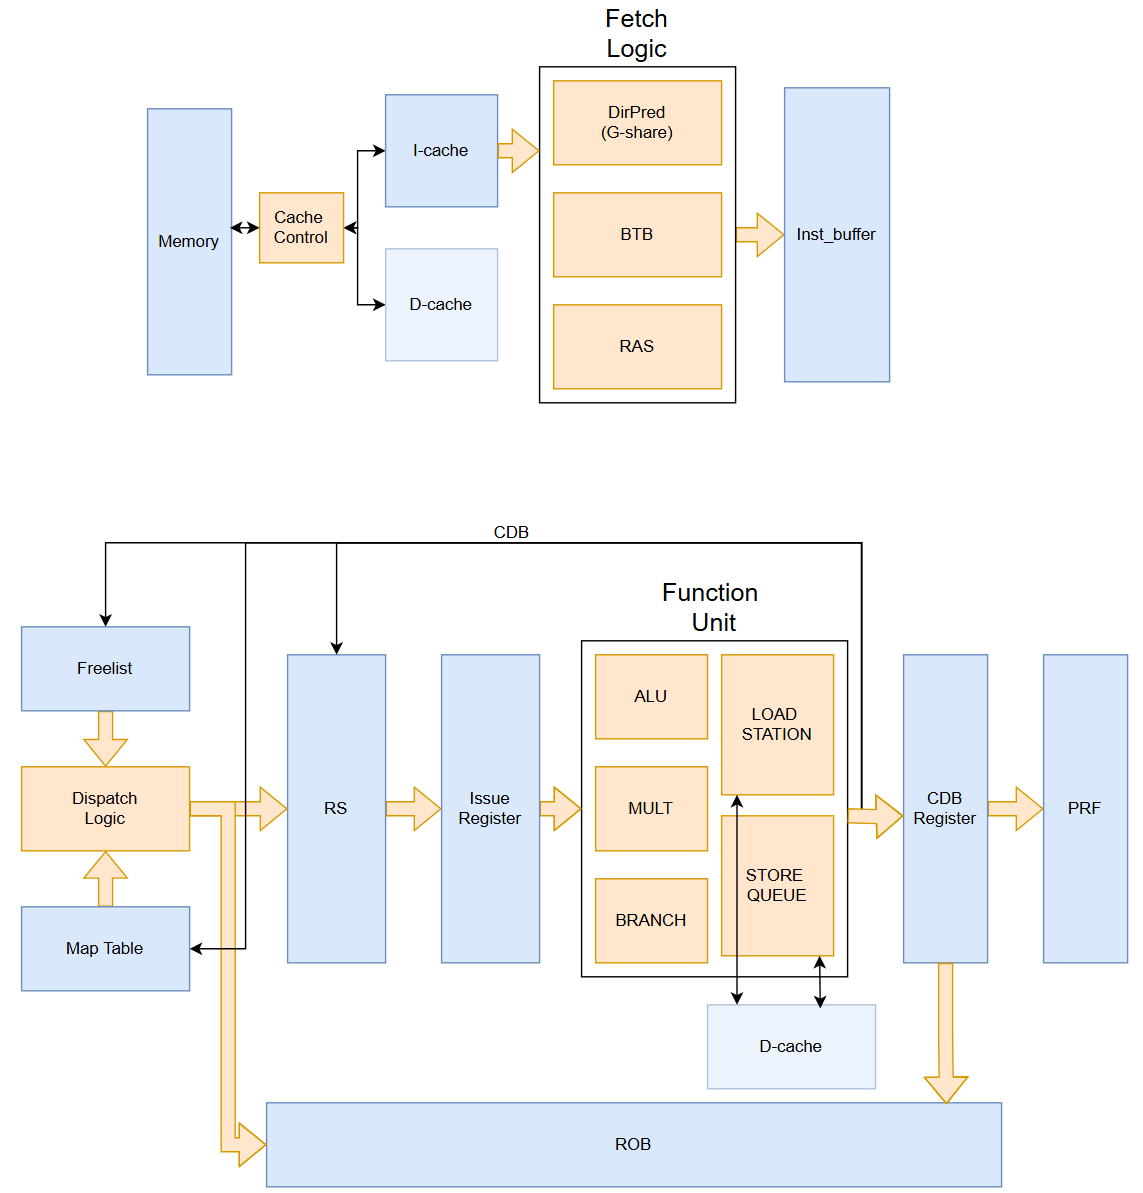
\includegraphics[width=0.3\textwidth]{figures/overall.png}}
\caption{High-level design.}
\label{fig:high_level}
\end{figure}


In the diagram, blue blocks represent registers and orange ones represent combination logic. Meanwhile, we've also implemented other advanced features. 

\subsection{List of Features}

\subsubsection{Features Present in the Final Design}

\begin{itemize}
  \item N-way superscalar
  \item Early Branch Resolution
  \item Early Tag Broadcast
  \item G-Share Branch Predictor
  \item Return Address Stack
  \item Instruction Prefetching
  \item Dual-ported, banked i-cache
  \item Non-blocking d-cache
  \item Out-of-order issue of mem requests (loads)
  \item Data forwarding from stores to loads
  \item Testing \& Debugger: see corresponding sections
\end{itemize}

\subsubsection{Features not in the Final Design}

We made explorations in various directions. Some features are not incorporated in our final submission, either due to performance reasons or time constraints. Here is a list of them, and where to find them:

\begin{itemize}
  \item Advanced Predictors: TAGE-like, Perceptron, and CNN. Implemented on branch "bp-TAGE2" (TAGE-like), branch "bp-CNN" (1-layer CNN), branch "bp-n-layer-CNN" (n-layer CNN), and "perception" (perceptron, note the typo in branch name), file "verilog/dirPred.sv"
  \item Associative d-cache. Implemented on branch "associative\_cache" (2-way) and "fourway" (4-way), file "verilog/dcache.sv"
  \item Issuing instructions in program order. Implemented on branch "rs-age-logic", file "verilog/rs.sv"
\end{itemize}

\subsection{Basic Components}
\subsubsection{Reservation Station}

We've designed a 16-entry Reservation Station (RS). It will receive the instruction from dispatch and record the new tag designated by Free List. Also, it will keep updating the readiness of the source tag from Common Data Bus (CDB) in order to prevent the read after write (RAW) problem. 

Meanwhile, it will issue the instruction that has all source registers ready to the Issue Register and Function Units. 

\subsubsection{Re-Order Buffer}

Our Re-Order Buffer (ROB) is a 32-entry FIFO table. It has two pointers of head and tail, to keep track of the FIFO list. During the dispatch stage, every instruction will be allocated at the end of the list in ROB. Every instruction will be marked complete when it leaves the complete stage. Since we want to seek a precise state, instructions are retired in order. ROB will send the old tag of that instruction to Free List to recycle it. 

\subsubsection{Freelist and maptable}

These two modules are used to keep track of the register renaming state. We have 64 tags and PRF in total. Free List is to keep the unused tags and allocate these tags to the newly dispatched instructions. It also recycles the old tags of retired instructions. Map Table records the mapping of architecture register with the tag. It will also keep track of the readiness of each tag. Once receives a tag in the CDB, it will mark that tag as ready. 

\subsubsection{Function Units}

We totally have 3 ALUs, one 4-stage mult unit, one branch unit, one load unit, and one store unit. Mult unit is responsible for all multiplication instructions and ALUs for other arithmetic instructions. Branch unit contains a comparator to resolve the branch result and an adder to calculate the target PC. It is also where JAL and JALR instructions go. Load unit and store unit both contain one adder, which is responsible for calculating the memory address they want to access. These results will be sent to load station and store queue for further processing. 


\subsection{ETB}
Because of the limited width of Common Data Bus, after leaving the execute stage, all calculated results will be written into to CDB register, waiting for arbitration. In the next cycle, the arbiter will choose several to get into the CDB and write back to the PRF. The CDB contains the tag that has finished writing back. 

However, with ETB feature, the arbitration will happen one cycle early, and the tag will be broadcast one cycle early. For one stage units (ALU, branch and store unit), they will run for the CDB. If they succeed, they will be issued. If not, they will still stall in the RS instead of the execution stage. Meanwhile, mult unit will be running for CDB one cycle earlier (i.e. last but one stage) and will only continue to final stage if it is granted by CDB arbiter. As a result, we need to bypass the data in CDB reg to the issue stage. 

\subsection{Early Branch Resolution (EBR)}
In the basic pipeline design, branch instructions are resolved during the retire stage. If a branch instruction is found to have been mispredicted, all subsequent instructions in the pipeline are flushed, and the processor begins fetching from the correct target address. However, the outcome of a branch can be known as early as the execution stage. Resolving branches immediately after execution reduces the performance cost of mispredictions and improves overall throughput. This technique is referred to as Early Branch Resolution (EBR) in our design.

Because instructions are issued out of order, both preceding and succeeding instructions relative to the resolved branch can be present in the pipeline. To manage this, each instruction is tagged with a branch index, indicating its dependency on unresolved branches. This allows the system to selectively squash only the instructions along the mispredicted path, while preserving those that precede the branch in program order.

When a branch instruction is fetched, an entry in the branch stack is allocated, and the index of this entry is used as its branch index (b-index). Each instruction is also assigned a branch mask (b-mask), which records the indices of all currently unresolved branches. This mechanism is illustrated in Fig. \ref{EBR-fetch}.

\begin{figure}[htbp]
\centerline{
\includegraphics[width=0.6\columnwidth]{Design/EBR-fetch}}
\caption{Marking instructions with EBR logic. }
\label{EBR-fetch}
\end{figure}

When a branch is resolved, its outcome—whether the prediction was correct—and its branch index are broadcast to all pipeline stages holding instructions. If it was a misprediction, all instructions with the corresponding index in their b-mask are squashed. If the prediction was correct, the corresponding index is cleared from each instruction’s b-mask, indicating they no longer depend on that branch.

\subsection{N-Way Superscalar Design}
In a traditional 5-stage pipeline, each stage handles at most one instruction per cycle. To increase throughput, our processor adopts a superscalar architecture, which allows multiple instructions to progress through each stage simultaneously. We implement an N-way superscalar design, where N parameterizes the maximum number of instructions per stage.

In ideal conditions, when there are no inter-instruction dependencies, performance can theoretically scale by a factor of N. This approach boosts instruction-level parallelism and enhances overall processor efficiency.


\subsection{Cache}
Accessing main memory in our design incurs a 100ns latency. To mitigate this overhead, the processor employs caches that exploit spatial and temporal locality by storing recently accessed data. We implement separate caches for instructions and data, as their access patterns differ and exhibit minimal overlap.

\subsubsection{Instruction Cache}
The instruction cache (i-cache) is direct-mapped, banked, and supports prefetching. It is banked to enable parallel access to two memory blocks, supporting up to 4-way instruction fetch.

A stream buffer is employed to prefetch the next memory line while waiting for the current memory request to complete. The fetched data is temporarily stored in the stream buffer. If a requested address hits in the prefetch buffer, the corresponding block is deemed useful and promoted into the i-cache. If a request is made for an address not captured by the prefetch mechanism, the entire stream buffer is flushed, and prefetching resumes from the new address.

\subsubsection{Data Cache}
The data cache (d-cache) is a basic direct-mapped cache. It incorporates a Miss Status Holding Register (MSHR) to support non-blocking behavior. The MSHR stores requests that miss in the cache, allowing subsequent requests to proceed without stalling the pipeline. When the requested data is retrieved from memory, it is broadcast to fulfill the pending requests corresponding to that MSHR entry. This design enables the cache to issue useful memory requests every cycle without being bottlenecked by a single outstanding miss.

\subsection {Load Station and Store Queue}

Since the memory access has a long latency and withdrawing a memory write-back is quite hard, we need a store queue (SQ) that can monitor all store instructions before retire to keep the memory write-back in order. We also need a load station that can support out-of-order load issues and complete. Our strategy is non-speculative. You can see our design in Fig. \ref{fig:lsq}. SQ is a FIFO and load station is not in order. 

\begin{figure}[htbp]
\centerline{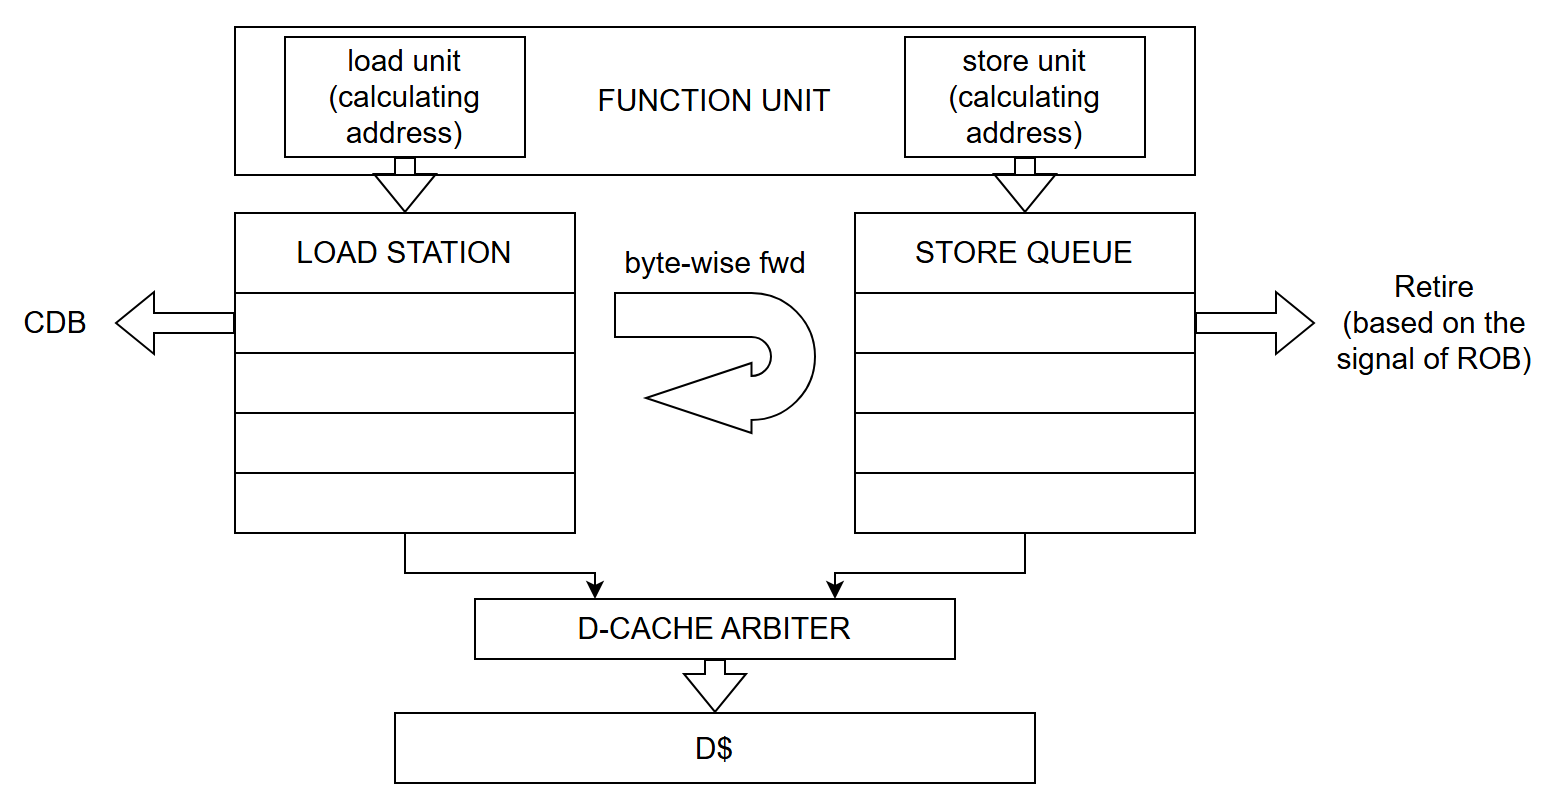
\includegraphics[width=0.3\textwidth]{figures/load_station.png}}
\caption{Load station and store queue layout.}
\label{fig:lsq}
\end{figure}

\subsubsection{Store Queue}

A store instruction will be allocated in SQ when dispatched. Then, after it is executed, the memory address and data will be stored in SQ. Then, it will send the store request to D-cache when it is retired in the ROB. If the D-cache is meeting a structural hazard, this cycle's attempt will fail, the retire will be stalled and it will repeat in the next cycle. 

\subsubsection{Load Station}

A load instruction receives an SQ (Store Queue) position indicating the tail, which helps track all prior store instructions when dispatched. The load is issued only when its source register is ready and all preceding stores have computed their addresses. This ensures at least one valid data source—either memory or the SQ. It leaves the station when gets the data and then goes to the complete stage. 

In the load station, it first gets forwarding data from the SQ before requesting data from the cache. The load station operates as an FSM. If a structural hazard with the D-cache prevents the request, it retries until successful. Upon receiving a cache response, a hit completes the operation, while a miss keeps the load waiting in the station.

To guarantee correct forwarding, we implement byte-wise forwarding. The logic treats the cache line as a unit: the SQ returns an entire cache line (shared with the load) along with a mask specifying forwarded bytes. When the load later receives cache data, it masks out these bytes to ensure correctness. 


\subsection{Branch Prediction}
Branch target addresses are predicted during the fetch stage, enabling the processor to fetch from the predicted target in the next cycle. We employ a GShare direction predictor, which leverages global history and program patterns to improve prediction accuracy. To predict target addresses, we employ a branch target buffer for general cases and a return address stack specifically for return statement predictions.

To balance complexity and latency, the predictor generates at most one branch prediction per cycle. This ensures efficient execution without incurring high prediction overhead.

